\multiproblem{0}{
\begin{enumerate} 
\item{A configuration of a system is given below. 
            \begin{center}
                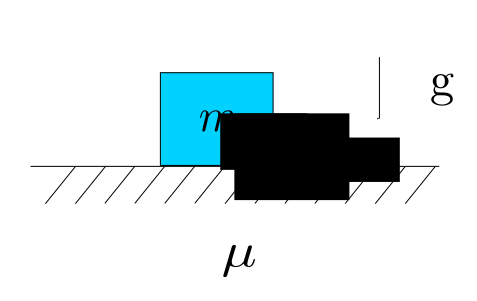
\includegraphics[scale=0.4]{noah1.pdf}
            \end{center}
Given that the block has a mass $m=10$ kg, and the coefficient of friction between the block and the surface is $\mu=1$:}
     \begin{enumerate} 
        \item{What is the normal force on the block? \A{\\$F_N=$Weight of block $=mg=98.1$N}
        }
        \item{If an external horizontal force of 10 N is applied to the block will it remain in equilibrium? \A{\\Yes: $F_f\leq\mu F_N=\mu m g =100$N$>10$N}
        }
        \item{What is the maximum horizontal force that can be exerted upon the block without it moving? \A {\\$F_H=F_f\leq 98.1$N and so the maximum force is 98.1N}
        }
        \item{Suppose we have a different surface roughness and measure that the largest horizontal force we can exert upon the block without it moving is 25N. What is the new value for the coefficient of friction in this case? \A{\\As forces are balance in this equilibrium $F_{H_{max}}=F_{f_{max}}= \mu m g$. And so by rearranging $\mu=\frac{F_H}{mg}=\frac{1}{4}= 0.25$}	
        } 
     \end{enumerate}
\end{enumerate}
}

\multiproblem{1}{Masses on springs
\begin{enumerate}
\item The figure below shows a configuration of a mass (which we will treat as a point particle) hanging on a light spring. The particle has mass $m$, and the distance of the particle from the ceiling is $y$. The spring has the following properties: spring constant $k$ and natural length $l$
            \begin{center}
                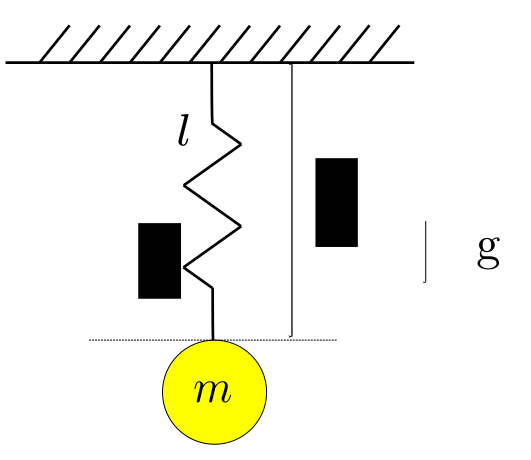
\includegraphics[scale=0.4]{noah2.pdf}
            \end{center}.
	\begin{enumerate}
	\item{ Firstly, justify that the units of the spring constant are N/m with the use of Hooke's Law. \A {\\Force (N) = constant $\times$ extension (m), and so constant= Force (N) / extension (m)}
	}
	\item{Find the distance $y$ given that $m=10$ kg, $k=200$ N/m and $l=1$ m. \A{\\Restorative spring force $F_s=k(y-l)$, weight $F_G=mg$, forces balanced and so $F_s=F_G=k(y-l)=mg$, and so $y=\frac{mg}{k}+l=0.5+1=1.5$m}
	}
	\item{Now instead, find a general expression for the distance $y$ in terms of the parameters $m,l,g,k$. \A {\\see above}
	}
	\item{Sketch the distance $y$ as a function of $k$ and label key features (you can use $m=10$ kg and $g=10$ m/s$^2$).%\A 
	}
	\end{enumerate}
	
\item The figure below shows a configuration of a block of mass $m$ on a surface. 
            \begin{center}
                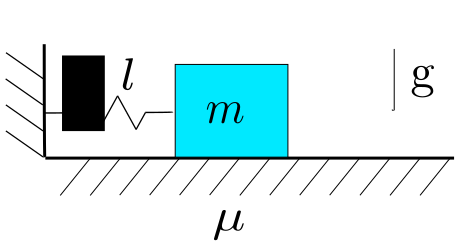
\includegraphics[scale=0.4]{noah3.pdf}
            \end{center}
The block is also attached by a spring (with spring constant $k$ and natural length $l$) to the wall. The distance of the block from this wall is given by $d$. Given that $m=1$ kg and $l=1$ m:
	\begin{enumerate}
	\item{ What is the value of the normal reaction force on the block? \A {\\Normal force and weight are balanced $F_n=mg=100$N}
	}
	\item{Assuming that the surface is smooth ($\mu=0$) and the spring constant $k>0$, state the distance $d$ at which the system is in equilibrium. \A{\\The horizontal forces must balance so the spring force $F_s=k(d-l)$ is equivalent to the frictional force $F_f\leq\mu F_N$, since $\mu=0$ this frictional force must also equal 0 and so $F_s=k(d-l)=0$ which implies $x=l$m}
	}
	\item{Assume now that the surface is rough and that the coefficient of friction $\mu=1$. Furthermore, the spring constant is known to be $k=40$ N/m. What is the range of values of $d$ for which the block may be in equilibrium? Hint: should be in the form $d_1\leq d\leq d_2$ \A {\\$1-0.25\leq d\leq 1+0.25.$}
	}
    %\item{If Repeat the previous question for general $\mu,l,g,$ and $k$ \A{\\$l-mg/k \leq d \leq l+mg/k$}
    \item{Using the same method as in part iii., derive a general expression for the range of values of $d$ for which the block is in equilibrium in terms of unknown parameters $\mu,l,g,$ and $k$.
}
	\end{enumerate}	
\end{enumerate}

}

\multiproblem{2}{Masses on slopes
\begin{enumerate}
\item Consider a mass $m$ on a slope at angle $\alpha$ to the horizontal. Assume the surface of the slope has a coefficient of friction $\mu$. 
            \begin{center}
                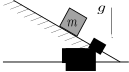
\includegraphics[scale=0.4]{fig_1.pdf}
            \end{center}
            \begin{enumerate}
            	\item Draw a free-body diagram of the system
		\item If mass $m = 10$ kg and angle $\alpha = \pi/6$, determine the maximum value of the friction force, $F$, which ensures the system is in equilibrium. {\it Assume $\mu =1$}.
		\item Derive an inequality in terms of parameter $\alpha$ that defines the range of values of $\mu$ for which this system will remain in equilibrium. This should be of the form $\mu \geq f(\alpha)$.
		\A{\\We need to use Coulomb Friction: $|F| \leq \mu N$.}
		\A{\\From the free body diagram: $N= mg\cos(\alpha)$ ($1$), $F = mg\sin(\alpha)$ ($2$).}
		\A{\\Using $2$ and Coulomb Friction, we have $|mg\sin(\alpha)| \leq N \mu$, therefore (using $1$ to eliminate $N$), $\mu \geq |\tan(\alpha)|$}
             	\item Sketch the variation in the maximum value of $\mu$ as a function of angle $\alpha$ for the range $0 \leq \alpha \leq \pi/2$. Interpret your sketch for large $\alpha$ ($			\alpha \to \pi/2$). 
            \end{enumerate}
            
\item Consider the system in question 2.b placed on a slope that makes an angle $\alpha$ to the horizontal, such that the central axis of the spring is parallel to the surface of the slope. Assume the surface of the slope has a coefficient of friction $\mu$.
            \begin{center}
                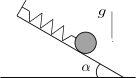
\includegraphics[scale=0.4]{fig_2.pdf}
            \end{center}
	\begin{enumerate}
		\item Draw a free body diagram of the system.
		\item If the slope is at an angle $\alpha = \pi/6$ to the horizontal, $k = 1$ N/m, $x = 2$ m and $m = 10$ kg, find the minimum value of the friction coefficient, $\mu$, that 				ensures the mass is 	stationary. 
		\item Derive an inequality in terms of parameters $m$, $g$, $\alpha$, $k$, and $\mu$,  that defines the range of values of $x$, the extension of the spring, for 					which this system is in equilibrium.
		\A{\\We need to use Coulomb Friction: $|F| \leq \mu N$, where $F$ is the net force acting parallel to the slope. }
		\A{\\From the free body diagram: $N= mg\cos(\alpha)$ ($1$), $F = mg\sin(\alpha) - kx$ ($2$).}
		\A{\\Using $2$ and Coulomb Friction, we have $|mg\sin(\alpha) - kx| \leq mg\cos(\alpha) \mu$.}
		\A{\\Rewriting: - $mg\cos(\alpha) \mu \leq mg\sin(\alpha) - kx \leq mg\cos(\alpha) \mu$.}
		\A{\\Rearranging for $x$: $- \frac{mg}{k} (\cos(\alpha) + \sin(\alpha)) \leq -x \leq \frac{mg}{k} (\cos(\alpha) - \sin(\alpha))$}
		\item If the spring is replaced by one which is stiffer, how does this affect the range of extensions for which the mass is stationary? Use a sketch to demonstrate this result. {\it 			Hint: Try plotting $x$ vs $k$ and shading the region defined by the inequalities.}
	\end{enumerate}
\end{enumerate}
}

\multiproblem{3}{Systems of 2 masses
\begin{enumerate}
\item 2 masses $m_1$ and $m_2$ are connected by a spring of stiffness $k_2$ and natural length $L_2$. Mass $m_1$ is also connected to a wall by a spring of stiffness $k_1$ and natural length $L_1$. The surface on which the masses are resting has a coefficient of friction $\mu$.
            \begin{center}
                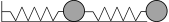
\includegraphics[scale=0.4]{fig_3.pdf}
            \end{center}
	\begin{enumerate}
	\item Draw a free body diagram for each mass.
	\item If $m_1 = m_2 = 10$ kg, $k_1 = k_2 = 1$ N/m, $x_1 = 2$ m, $x_2 = 0.5$ m, $L_1 = 2$ m and $L_2 = 4$ m, find the minimum value of $\mu$, the coefficient of friction, that ensures mass $m_1$ is stationary.
	\item Find two inequalities for the range of values of $\mu$, the coefficient of friction, that ensure the system is in equilibrium. 
	\A {\\From the free body diagrams we have: $N_1 = m_1g$, $N_2 = m_2g$, $F_2 = k_2x_2$ , $F_1 = k_1(x_1-x_2)$.}
	\A {\\Applying Coulomb Friction to each mass we obtain: $|\frac{k_1}{m_1g}(x_1 - x_2) |\leq \mu$ and $|\frac{k_2 x_2}{m_2g}| \leq \mu$.}
	\item {\it Hard question} If $m_2 = \beta m_1$, $x_2 = \gamma x_1$ and $k_2 = \delta k_1$, using the expressions from part ii, sketch a graph for $\mu$ as a function of $\beta$. Sketch another graph for $\mu$ as a function of $\delta$. How does this differ from a system of only one mass (question 2.b)?
	\A{\\Using the expressions derived above and substituting for $m_2$, $k_2$ and $\epsilon_2$, we obtain:}
	\A{\\$|\frac{k_1x_1}{m_1g}(1 - \gamma) |\leq \mu$, }
	\A{\\$|\frac{\delta k_1 \gamma x_1}{\beta m_1g}| \leq \mu$}
	\end{enumerate}
	
\item{The following figure shows a configuration of masses and pulleys. Both the block and the particle have mass $m=1$kg
            \begin{center}
                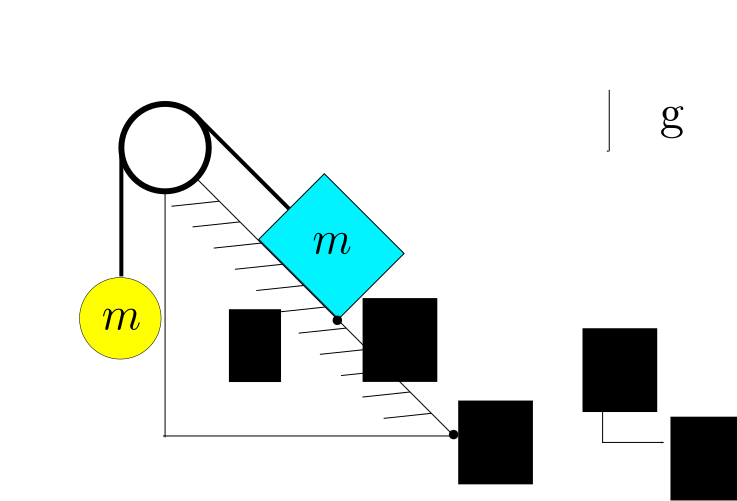
\includegraphics[scale=0.4]{noah4.pdf}
            \end{center}}
\begin{enumerate}
	\item{Draw free body force diagrams for both the block and the particle}
	\item{Point $B$ is at position $-1$i$+1$j from point $A$. If $m=1$ kg and $\mu=1$ can the system be in equilibrium?\A {\\Yes: If in equilibrium the forces are balanced on the particle and so the tension in the pulley string is equivalent to the weight of the particle ($T_p=mg$). Now looking at the block we can see that the frictional force must act on the block in the direction down the slope. So assuming equilibrium, resolving the forces parallel to the slope we have $T_p=mg=mg$sin$(\theta) + F_f$ where $theta$ is the angle of the slope. This angle of the slope with the horizontal can be found to be $theta=45^o=\pi/4$rad from the position vector. Furthermore, the frictional force is given by the inequality $F_f\leq \mu F_N$ where $F_N$ is the normal force (perpendicular to the slope). This can be found to give $F_f\leq \mu  mg$cos$(\theta)$. If we substitute this into the earlier equation we find $mg(1-$sin$(\theta))=F_f\leq\mu  mg$cos$(\theta)$ which simplifies to $1-$sin$(\theta)\leq$cos$(\theta)$ which is easily shown to be true.} 
	}
	\item{What is the critical value of $\mu$ (the smallest value such that the system may still be in equilibrium)? 
	\A {\\At this critical point $F_f=\mu F_n$ and so it can be found in the same way as before that $\mu mg$cos$(\theta)+mg$sin$(\theta)=mg$ which can be easily rearranged to give 		$\mu=(1-$sin$(\theta))/$cos$(\theta))=\sqrt{2}-1\approx 0.41$}
	}
\item{Now give an expression for critical value of $\mu$ for the system when the slope makes an angle $\alpha$ to the horizontal.	
	\A{\\$\mu=(1-$sin$(\theta))/$cos$(\theta))$ See above}
}
\end{enumerate}

\item Two masses, $m_{1}$ and $m_{2}$ are connected by a spring with stiffness $k$ attached to a light inextensible string running smoothly over a pulley, as shown below.
            \begin{center}
                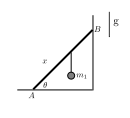
\includegraphics[scale=1.8]{fig_4.pdf}
            \end{center}
	    Mass $m_{2}$ rests on a slope at unknown angle $\theta$. 
            \begin{enumerate}
            \item Draw free body diagrams for both masses. Find the two horizontal and vertical force balance equations for each mass.
            \item Assuming angle $\theta = \pi/6$, $m_1 = 10$ kg, $m_2 = 5$ kg, $k = 2$ N/m and extension $x = 1$ m, find the minimum value  of $\mu$ such that the system is in static equilibrium. 
	    \item Suppose $m_{1}$ and $m_{2}$ are known. If there is no friction acting on the slope, for which values of $\sin(\theta)$ is there a unique solution?
	    \item Now suppose there is friction, and that $m_{1}$, $\mu$ and $\theta$ are all known. What is the set of values of $m_{2}$ for which static equilibrium is possible? What is the corresponding extension of the spring,~$x$? Can $m_{2}=0$ and what is the condition in $\mu$ and $\theta$ for this to occur?  
	    \A {\\$m_2g = T$, $m_1g\cos(\theta) = N$, $T=kx - m_1g\sin(\theta)$}
	    \A {\\$m_2g = k(x-L) - m_1g\sin(\theta)$}
	    \A {\\$|F| \leq N\mu \to |m_2g - kx+ m_1g\sin(\theta)| \leq \mu m_1g\cos(\theta)$}
	    \A {\\$- \mu m_1g\cos(\theta) \leq m_2g -kx + m_1g\sin(\theta) \leq \mu m_1g\cos(\theta)$}
	    \end{enumerate}
 \end{enumerate}
}